\newpage
\chapter{Приближени пресмятания - подходи, методи, алгоритми}
\label{chapter10}
\thispagestyle{empty}

В изчислителната математика се открояват две основни направления – точните числени пресмятания и приближените числени пресмятания\index{приближени пресмятания}. Точни числени пресмятания\index{точни числени методи} се извършват в ситуации в които обемът на задачата позволява изчисленията да се осъществят в приемлив интервал от време. В реалната практика често поставяните задачи значително нарастват като обем и тяхното пресмятане с точени числени методи става неприемливо по отношение на нужното време за пресмятане. В такива ситуации се прибягва до множеството разработени методи за приближени пресмятания\index{приближени числени методи}. По отношение на програмния продукт R, ще бъдат разгледани някои от най-популярните методи за приближени числени пресмятания, а именно Монте-Карло симулации, генетични алгоритми и изкуствени невронни мрежи.

\section{Монте-Карло методи}

В средата на XX век, във връзка с разработването на първите ядрени оръжия, са разработени група методи за приближени пресмятания, които залагат на способ за генериране на голямо количество случайни числа и последващата им статистическа обработка. Монте-Карло методите\index{Монте-Карло методи} намират най-голямо приложение в оптимизационни задачи, числено интегриране и генериране на семпли за специфични вероятностни разпределения. Монте-Карло методите могат да се използват за решаването на всяка задача, която има представяне в термините на вероятности и статистика. 

Има вариации в реализацията на Монте-Карло методите, но те в общия случай следват няколко добре дефинирани стъпки:

1. Определяне на област от допустими стойности;

2. Генериране на извадка от случайни числа в предварително дефинираната област;

3. Извършване на точни пресмятания с така генерираните случайни числа;

4. Обобщаване на резултатите от извършените пресмятания.

\begin{figure}[h!]
  \centering
  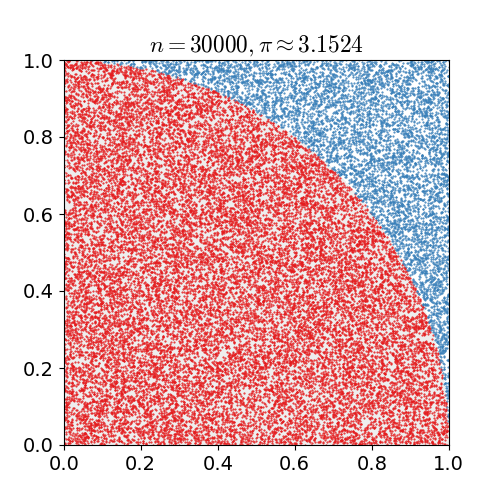
\includegraphics[width=0.8\linewidth]{pic0060}
  \caption{Пресмятане на числото $\pi$ с Монте-Карло метод}
\label{figure0060}
\end{figure}
\FloatBarrier

Един от най-популярните примери за Монте-Карло пресмятане е приближеното изчисление на числото $\pi$ (Фиг. \ref{figure0060}). За тази цел една четвърт от окръжност се представя с обгръщащия я квадрат. Съотношението между площите на квадрата и на четвъртината окръжност е $\pi/4$. За да се апроксимира стойността на числото $\pi$ с Монте-Карло метод се изпълняват следните стъпки:

1. Изчертаване на квадрат и четвъртина окръжност вписана в него;

2. Генериране на случайни равномерно разпределени числа, като координати (x,y двойки) в описаната допустима област;

3. Изброяване на точките с координати x,y които са на разстояние 1 от центъра на четвърт окръжността; 

4. Съотношението между точките в четвърт окръжността и общия брой точки е $\pi/4$, което умножено по 4 дава приближена стойност за числото $\pi$. 

При тази процедура за приближено пресмятане е важно да се вземат под внимание два много важни фактора:

1. Ако генерираните случайни числа не са равномерно разпределени, това ще доведе до невярна апроксимация за търсената стойност;

2. Генерирането на малък брой координати за точки в дефиниционната област води до ниско надеждна стойност за апроксимация, което означава, че колкото по-голям обем е извадката от случайни числа, толкова по-надеждни резултати за апроксимация.

\begin{lstlisting}[caption=Монте-Карло пресмятане, label=listing0175]
library( MonteCarlo )

mode <- function(x) {
	values <- unique(x)
	return( values[which.max(tabulate(match(x, values)))] )
}

experiment <- function(n, d){
	x <- sample(6,n,TRUE)

	for(i in 2:d) {
		x <- x + sample(6,n,TRUE)
	}

	return( list("mean"=mean(x), "median"=median(x), "mode"=mode(x)) )
}

result <- MonteCarlo(func=experiment, nrep=1000, param_list=list("n"=c(10, 50, 100, 150, 200),"d"=c(1,2,6)))

summary( result );

MakeTable(output=result, rows=c("d"), cols=c("n","list"), digits=2, include_meta=FALSE)
\end{lstlisting}

Към програмния продукт R е създаден отделен пакет (автор Christian Hendrik Leschinski) за извършване на Монте-Карло пресмятания, наречен „MonteCarlo“ (Листинг \ref{listing0175}). 

За демонстрация на възможностите, които R дава при Монте-Карло симулации е представено сравнение между средната, медианата и модата за вероятностно разпределение на сумата от $n$ зара. Тъй като R не предлага функция за пресмятане на мода е необходимо тази функция да бъде предварително дефинирана (Листинг \ref{listing0175}).

В пакета $MonteCarlo$\index{Монте-Карло методи} основно се използват две функции - $MonteCarlo$ и $MakeTable$. Функцията $MonteCarlo$ има за основна задача генерирането на множеството експерименти в процеса на симулацията. Най-важният параметър за тази функция е функционален обект, който описва единичен експеримент. В програмния език R функционалните обекти по своята същност представляват потребителски дефинирани функции. В предложения пример функционалният обект се нарича $experiment$, а функцията която представлява получава два входни параметъра $n$ и $d$. Потребителят на пакета $MonteCarlo$ сам може да избира какъв брой параметри да има функцията за единичен експеримент. В настоящия пример $n$ определя броят случайни числа, които да бъдат генерирани (размер на случайната извадка), а $d$ определя колко зара ще участват във формирането на крайния резултат. При предишни примери бе показано, че вероятностното разпределение на един зар е равномерно, на два зара триъгълно, а при достатъчно много зарове разпределението клони към нормалното. В този пример се разглеждат разликите между средната, медианата и модата за 1, 2 и 6 зара.

Към функцията за единичен експеримент има следните изисквания: 1. Аргументите а бъдат скаларни стойности; 2. Върнатата стойност от функцията да бъде списък с именувани или неименувани скаларни стойности. Потребителската функция за единичен експеримент се изпълнява в текущото работно пространство и поради тази причина всички нужни библиотеки, променливи с данни и помощни функции трябва да са заредени предварително. 

Вторият важен аргумент на функцията $MonteCarlo$ е $param_list$ и трябва да изпълнява следните изисквания: 1. Трябва да е списъчна структура; 2. Елементите на списъка трябва да са именувани и имената да съответстват на имената използвани за параметри в потребителската функция за единичен експеримент; 3. Всеки елемент в списъка е вектор със скаларни стойности; 4. Списъкът съдържа точно толкова на брой елементи, колкото са параметрите на потребителската функция за единичен експеримент. 

Последният задължителен аргумент на функцията $MonteCarlo$ е $nrep$ и той определя колко пъти ще бъде изпълнен Монте-Карло експериментът. В представения пример (Листинг \ref{listing0175}) се изпълняват хиляда повторения за три възможни комбинации от зарове, при пет различни броя за хвърлянето на тези зарове, а именно 10, 50, 100, 150 и 200. 

\begin{table}[h]
\centering
\resizebox{ 1 \textwidth}{!}{%
\begin{tabular}{ rrrrrrrrrrrrrrrrrrr }
\hline\hline\\\\
 list && \multicolumn{ 5 }{c}{ mean } &  & \multicolumn{ 5 }{c}{ median } &  & \multicolumn{ 5 }{c}{ mode } \\ 
d/n &  & 10 & 50 & 100 & 150 & 200 &  & 10 & 50 & 100 & 150 & 200 &  & 10 & 50 & 100 & 150 & 200 \\ 
 &  &  &  &  &  &  &  &  &  &  &  &  &  &  &  &  &  &  \\ 
1 &  & 10.50 & 10.48 & 10.49 & 10.50 & 10.50 &  & 10.52 & 10.50 & 10.48 & 10.50 & 10.52 &  & 10.48 & 10.50 & 10.42 & 10.49 & 10.53 \\ 
2 &  &  7.01 &  7.00 &  7.00 &  7.01 &  6.99 &  &  7.02 &  7.01 &  7.00 &  7.00 &  7.00 &  &  7.03 &  7.04 &  6.98 &  6.98 &  6.99 \\ 
6 &  & 20.94 & 21.03 & 21.00 & 21.01 & 21.00 &  & 20.90 & 21.01 & 20.99 & 21.00 & 21.00 &  & 20.86 & 20.98 & 21.04 & 21.00 & 20.97 \\ 
\\
\\
\hline\hline
\end{tabular}%
}
\caption{Сравнение на средна, медиана и мода за експеримент със зарове}
\label{table0005}
\end{table}

За визуализация на получените резултати от функцията $MonteCarlo$ се използва функцията $MakeTable$. На функцията $MakeTable$ се подава резултата от симулацията и тя генерира таблица с резултати в $LaTeX$ формат (Таб. \ref{table0005}).

Функцията $MakeTable$ дава множество възможности, но само три от аргументите й са задължителни. На аргумента $output$ се присвоява резултата от изпълнението на функцията $MonteCarlo$. Вторият и третият аргумент са $rows$ и $cols$, като те определят по какъв начин ще се организират табличните данни. В представения пример (Листинг \ref{listing0175}) по редове са организирани броя зарове участващи в единичен експеримент, а по колони са организирани броят хвърляния на заровете, групирани по вида статистика (средна, медиана или мода). 

Макар и незадължителен параметърът $digits$ е определен на 2, което дава по-добра прегледност на табличната визуализация. Също незадължителен параметърът $include_meta$ е установен на „лъжа“ с цел да не се генерират коментари с обобщаваща информация за извършената симулация. 

\section{Генетични алгоритми}


